\documentclass[12pt,phd,times]{pkmthesis}
\usepackage{amsmath,epsfig,graphicx,setspace,url,float}
\usepackage{pstricks,colortab,pifont}
\usepackage{lscape,multicol,multirow,longtable,subfigure}
\usepackage{cite,bm}
\usepackage[english]{babel}
\usepackage[small,bf]{caption}
\usepackage{csquotes}
\usepackage{threeparttable}
\usepackage{tikz}
\usepackage{pgfplots}
\pgfplotsset{compat=1.18}
\usetikzlibrary{shapes.geometric, arrows.meta, positioning, calc, patterns}
\usepackage{makecell}
\usepackage{booktabs}
\usepackage{enumitem}
\usepackage{listings}
\usepackage{xcolor}
\setlength{\textfloatsep}{1cm}
\normalem
\setlength{\abovecaptionskip}{8pt}
\setlength{\belowcaptionskip}{8pt}
\usepackage{hyperref}
\usepackage{extra_functions}
\input{pagesetup_pkm_middleside.tex}
\raggedbottom

% ---------- Listings styling ----------
\definecolor{codegreen}{rgb}{0,0.5,0}
\definecolor{codegray}{rgb}{0.5,0.5,0.5}
\definecolor{codepurple}{rgb}{0.58,0,0.82}
\definecolor{backcolour}{rgb}{0.96,0.96,0.96}
\lstdefinestyle{nice}{
    backgroundcolor=\color{backcolour},
    commentstyle=\color{codegreen},
    keywordstyle=\color{blue}\bfseries,
    numberstyle=\tiny\color{codegray},
    stringstyle=\color{codepurple},
    basicstyle=\ttfamily\footnotesize,
    breakatwhitespace=false,
    breaklines=true,
    captionpos=b,
    keepspaces=true,
    numbers=left,
    numbersep=5pt,
    showspaces=false,
    showstringspaces=false,
    showtabs=false,
    tabsize=2,
    frame=single
}
\lstset{style=nice}

% =============================================================================
\begin{document}
\setcounter{page}{1} \pagenumbering{roman}
\doublespacing

% ---------- Title page ----------
\thispagestyle{empty}
\pdfbookmark{Title}{Title}
\begin{center}
\fontsize{15.8pt}{19pt}\selectfont
{\textbf{Reducing Cross-Node Network Calls in Distributed Payment Systems via Thread-Level and Server-Local Caching\\}}
\vspace*{0.15in}
\emph{\large{A report submitted for end-term evaluation of the project for the award of}} \\
\emph{\large{Bachelor of Technology \\}}
\large{in \\}
\large{Information Technology\\}
\large{By}\\
\large{\textbf{Raman Kapoor : 2022BIT-XXX}} \\
\large{Under the Supervision of} \\
\large{\textbf{Dr.\ Vivek Kumar Singh}} \\

\end{center}
\begin{figure}[!h]
\centerline{\includegraphics*[width = 3cm]{FrontPages/ABV_IIITM_Logo.jpeg}}
\end{figure}
\centerline{\large{ABV-INDIAN INSTITUTE OF INFORMATION TECHNOLOGY }}
\centerline{\large{AND MANAGEMENT GWALIOR}} \vspace*{0.05in}
\centerline{\large{GWALIOR, INDIA}} \vspace*{0.05in}
\centerline{\large{2026}}

\thispagestyle{empty}

% ---------- Declaration / Certificate ----------
\clearpage
\thispagestyle{empty}
\pdfbookmark{Declaration}{Declaration}
\begin{center}
{\Large \bf DECLARATION}
\end{center}
\vspace{0.5cm}
\noindent I hereby certify that the work, which is being presented in the report/thesis, entitled REDUCING CROSS-NODE NETWORK CALLS IN DISTRIBUTED PAYMENT SYSTEMS VIA THREAD-LEVEL AND SERVER-LOCAL CACHING, in fulfillment of the requirement for end-term evaluation of the project for the award of the degree of Bachelor of Technology in Information Technology and submitted to the institution is an authentic record of my own work carried out under the supervision of Dr.\ Vivek Kumar Singh. I also cited the reference about the text(s)/figure(s)/table(s) from where they have been taken.

\vspace{1cm}

\begin{center}
\begin{tabular}{p{0.58\textwidth}p{0.4\textwidth}}
Dated:  & {\bf{Signature of the candidate}} \\
\end{tabular}
\end{center}
\vspace{1.5cm}
\noindent This is to certify that the above statement made by the candidate is correct to the best of my knowledge.

\vspace{1.5cm}

\begin{center}
\begin{tabular}{p{0.65\textwidth}p{0.4\textwidth}}
Dated: & {\bf{Signature of supervisor}} \\
\end{tabular}
\end{center}


% ---------- Acknowledgement ----------
\thispagestyle{empty}
\pdfbookmark{Acknowledgement}{Acknowledgement}
\begin{center}
{\LARGE \bf Acknowledgements}
\end{center}
\noindent
First and foremost, I would like to express my sincere gratitude to my supervisor, Dr.\ Vivek Kumar Singh, for his continual guidance, patience, and the freedom he gave me to explore the problem space on my own. His careful reading of every draft and his sharp, constructive feedback shaped both the technical depth and the presentation of this work. I am especially grateful for the way he encouraged me to engage with the question raised at the mid-evaluation rather than work around it; the contention layer that forms the new contribution of this report would not exist without that prompt.

I am also grateful to the engineering team at \emph{Juspay} for hosting the production environment in which the caching architecture was designed, deployed, and measured, and for the many design discussions that informed the safety boundaries described in this work. The opportunity to test ideas against real production traffic at the scale of millions of daily transactions was invaluable.

Finally, I would like to thank my family and friends for their patience and encouragement throughout this project, and the faculty and staff of ABV-IIITM Gwalior for the academic environment that made this work possible.

\begin{flushright}
\textit{\textbf{Raman Kapoor}}
\end{flushright}

\thispagestyle{empty}
\clearpage

% ---------- Abstract ----------
\thispagestyle{empty}
{\renewcommand{\baselinestretch}{1.5}
\begin{center}
{\bf{Abstract}}
\end{center}
\noindent Distributed payment systems serving millions of daily transactions face two intertwined challenges: redundant cross-node network calls that inflate p95/p99 tail latency, and concurrent contention on single, indivisible resources (e.g., a last available inventory unit, a unique reservation slot, a rate-limited gateway token) that must never be allocated twice. Each API request typically triggers 5--15 lookups to remote stores for merchant configurations, routing tables, feature flags and transaction metadata, even when much of this data is immutable within a request or over a short window. At the same time, the very caching layers introduced to reduce network hops can re-introduce correctness hazards: stale reads, lost updates, and double-allocations under high concurrency.

This report proposes an integrated two-layer architecture. The \textbf{caching layer} consists of (1)~a thread-level cache that eliminates redundant data fetches within a single request's execution context and (2)~a server-local cache that absorbs cross-request lookups for immutable, configuration-class data. The \textbf{contention layer} layers five complementary safety mechanisms over the cache: distributed locking with fencing tokens, atomic decrement via Redis Lua scripts, optimistic concurrency control with versioned cache entries, CRDT-based PN-Counters for eventually-consistent reservations, and single-flight request coalescing. Formal cache-safety boundaries govern which data classes are eligible for caching, and a decision matrix selects the right contention primitive per data class. Evaluation on a production payments platform handling roughly 68{,}000 cross-node operations per second shows a 4.1\% reduction in cross-node network calls at peak, an 11.2\% reduction in p95 latency and a 13.0\% reduction in p99 latency, with zero double-allocation incidents after the contention layer was rolled out. The combined approach is lightweight, requires no new infrastructure beyond a Redis cluster already present for caching, and is portable across language runtimes.
}

\thispagestyle{empty}
\clearpage

% ---------- TOC + LoF + LoT ----------
\dominitoc
\dominilof
\dominilot
\fancyhf{} \fancyhead[LE]{\bfseries\small{\leftmark}}
\fancyhead[RO]{\bfseries\small{\rightmark}}
\fancyfoot[CE,CO]{\bfseries\thepage}

\renewcommand{\baselinestretch}{1}
\pdfbookmark[0]{Index}{index}
\pdfbookmark[1]{Contents}{toc}
\fancyhead[LE]{\bfseries\small{Contents}}
\fancyhead[RO]{\bfseries\small{Contents}}
\tableofcontents
\clearpage

\pdfbookmark[1]{List of Figures}{lof}
\addstarredchapter{List of Figures}
\fancyhead[LE]{\bfseries\small{List of Figures}}
\fancyhead[RO]{\bfseries\small{List of Figures}}
\listoffigures
\clearpage

\pdfbookmark[1]{List of Tables}{lot}
\addstarredchapter{List of Tables}
\fancyhead[LE]{\bfseries\small{List of Tables}}
\fancyhead[RO]{\bfseries\small{List of Tables}}
\listoftables
\clearpage

% ---------- Body ----------
\fancyhf{}
\fancyhead[LE]{\bfseries\small{\leftmark}}
\fancyhead[RO]{\bfseries\small{\rightmark}}
\fancyfoot[CE,CO]{\bfseries\thepage}
\setcounter{page}{1} \pagenumbering{arabic}
\renewcommand{\labelenumi}{(\roman{enumi})}

\chapter{Introduction and Problem Statement}
\vspace{-1cm}
\noindent \rule{6.6in}{0.01in}
\section{Context}
Online payment platforms occupy a uniquely demanding position in the distributed-systems landscape: they must combine the throughput of large-scale web services, the latency budgets of interactive applications, and the correctness guarantees of financial ledgers. A single user-initiated transaction crosses several stateless API servers, a transactional database, and a number of supporting data stores --- typically a Redis cluster for hot configuration, a routing service for gateway selection, a risk-engine, and one or more downstream gateway integrations. Each component contributes to the end-to-end latency and to the overall correctness of the system.

\section{The Latency Problem}
Profiling on a production platform shows that a typical payment request triggers between five and fifteen \emph{cross-node network calls} during its lifecycle. Many of these calls are \emph{redundant}: they fetch the same merchant configuration, the same gateway routing table, or the same feature-flag value multiple times within the same request, or fetch effectively immutable data that has already been fetched by another concurrent request on the same node only milliseconds earlier. Each redundant call costs roughly 0.6--3.5\,ms of network round-trip time and contributes to load on the shared Redis cluster, amplifying tail latency at peak traffic \cite{kumar2024caching, qin2024tailcache}.

\section{The Concurrency Problem}
At the same time, certain operations involve \emph{single, indivisible resources}: the last unit of an inventory item, the only available time slot for a reservation, a unique gateway token issued under a per-second rate limit, or a single bank account being debited concurrently by two requests. Such operations cannot tolerate optimistic execution by both requests --- exactly one must succeed and the other must observe a definitive failure. During the minor evaluation of this work, an examiner posed the question: \emph{``If you cache state, how do you prevent two users from booking the same single piece?''} This paper takes that question as a central design constraint, rather than as an afterthought. Caching that satisfies safety boundaries (Section~\ref{sec:safety}) does not, by itself, resolve single-resource contention; a complementary contention layer is required.

\section{Problem Statement}
We address the following problem: \emph{In a distributed, stateless, high-throughput payment API, how can we (i) safely reduce the number of cross-node network calls per request via in-process caching, and (ii) guarantee that concurrent operations on single, indivisible resources cannot result in double-allocation, lost updates, or stale-cache-induced overselling --- all without introducing new infrastructure or sacrificing tail-latency improvements?}

\section{Contributions}
This paper makes the following contributions:
\begin{enumerate}[leftmargin=*]
    \item A formal \textbf{cache-safety boundary framework} (four criteria) that classifies data as cache-eligible or cache-ineligible by construction.
    \item A \textbf{two-tier in-process caching architecture} (thread-level + server-local) that operates entirely within the API server, requires no additional infrastructure, and reduces cross-node calls by 4.1\% at peak.
    \item A \textbf{contention layer} that integrates five complementary safety primitives --- distributed locking with fencing tokens, Redis Lua atomic decrement, OCC with versioned cache entries, PN-Counter CRDTs, and single-flight request coalescing --- and a decision matrix that selects the appropriate primitive per data class.
    \item A \textbf{production evaluation} on a payment platform handling $\sim$68{,}000 cross-node operations per second, demonstrating 11.2\% / 13.0\% reductions in p95 / p99 latency and zero double-allocation incidents over a 30-day post-deployment window.
    \item A \textbf{cross-runtime comparison} (Haskell, Java, Go, Rust, Node.js) showing how each tier and contention primitive maps onto idiomatic concurrency abstractions in each language.
\end{enumerate}

% =============================================================================
\label{chap:intro}

\chapter{Related Work}
\vspace{-1cm}
\noindent \rule{6.6in}{0.01in}
\section{Tail Latency and Distributed Caching}
The classical formulation of tail-latency amplification in large fan-out systems is due to Dean and Barroso, but recent comparative work has refined our understanding of how caching policies interact with the tail. Kumar et al.~\cite{kumar2024caching} present a 2024 comparative analysis of distributed caching algorithms across throughput, hit rate, and tail latency, finding that eventual-consistency caches achieve 3--5$\times$ higher throughput than strongly-consistent variants in read-dominated workloads. Qin et al.~\cite{qin2024tailcache} explore tail-optimised caching for high-fan-out inference workloads, demonstrating that policies designed for hit rate alone can paradoxically worsen p99 latency.

\section{In-Process and Multi-Tier Caches}
The trade-off between in-process and distributed caches has been examined extensively, both in industrial practice (Twitter, Cloudflare, Netflix) and in recent academic work. Tankoraphael~\cite{tankoraphael2026architecture} surveys 2026-vintage industry practice on multi-tier cache hierarchies and consistency, while DFUSE~\cite{wong2024dfuse} demonstrates that strongly-consistent write-back caching is achievable in distributed userspace file systems with carefully bounded staleness windows.

\section{Concurrency Control and Distributed Locking}
Concurrency control for single-resource contention has seen renewed attention. The recent arXiv survey of distributed locking~\cite{anonymous2025distlock} reports up to 68\% throughput improvements for modern distributed lock protocols over centralised baselines under high contention. \emph{OptiQL}~\cite{wang2024optiql} (SIGMOD 2024) re-examines optimistic locking for memory-optimised indexes; \emph{Motor}~\cite{wei2024motor} (OSDI 2024) introduces multi-versioning for distributed transactions on disaggregated memory; and Zhou et al.~\cite{zhou2025ccaas} (VLDB 2025) propose Concurrency-Control-as-a-Service, decoupling the CC layer from the storage engine.

\section{Atomic Operations and Lua Scripting}
On the Redis side, atomic decrement via Lua scripts has emerged as the de facto idiom for inventory-style operations. Recent industry write-ups~\cite{oneuptime2026lua, oneuptime2026inventory, dev2025redislua} document the pattern of bundling \texttt{GET}, conditional check, and \texttt{DECR} into a single Lua script to obtain serialised execution and prevent the classic read-modify-write race.

\section{Eventually-Consistent Counters and CRDTs}
Conflict-free replicated data types (CRDTs) provide a mathematically-grounded alternative to coordination for counters. Duncan~\cite{duncan2025crdt} provides a 2025 field-guide to CRDT primitives including PN-Counters; Shapiro et al.'s seminal work~\cite{shapiro2011crdt} remains the canonical reference, while recent applications to inventory and reservation systems are surveyed in~\cite{ably2024crdt, ijsoc2025inventory}.

\section{Single-Flight and Cache Stampede Mitigation}
Single-flight (also called request coalescing or de-duplication) is the most direct mitigation for cache stampedes. Vattani et al.'s XFetch paper remains the canonical academic reference for probabilistic early-refresh; recent practitioner write-ups~\cite{1xapi2026singleflight, oneuptime2026stampede, oneuptime2026coalescing} document the pattern in modern Go, Node, and Redis ecosystems. We contribute by integrating single-flight with our thread-level and server-local caches as a first-class primitive in the contention layer.

% =============================================================================
\label{chap:related}

\chapter{System Model and Background}
\vspace{-1cm}
\noindent \rule{6.6in}{0.01in}
\section{System Architecture}
The target system is a stateless, horizontally-scaled API tier written in Haskell, deployed across $N \approx 24$ application nodes behind a network load balancer. Each node serves on the order of 3{,}000 requests per second at peak. The application tier is supported by:
\begin{itemize}[leftmargin=*]
    \item A Redis cluster (six shards, three replicas) acting as the primary fast-path data store for merchant configuration, gateway routing, feature flags, and short-lived transactional state.
    \item A primary relational database (PostgreSQL) for the authoritative transaction ledger.
    \item A risk-decisioning microservice and a fleet of gateway-integration services.
\end{itemize}

\noindent Figure~\ref{fig:baseline-arch} shows the resulting topology and the cross-node call paths that this paper targets.

\begin{figure}[h]
\centering
\resizebox{0.95\textwidth}{!}{%
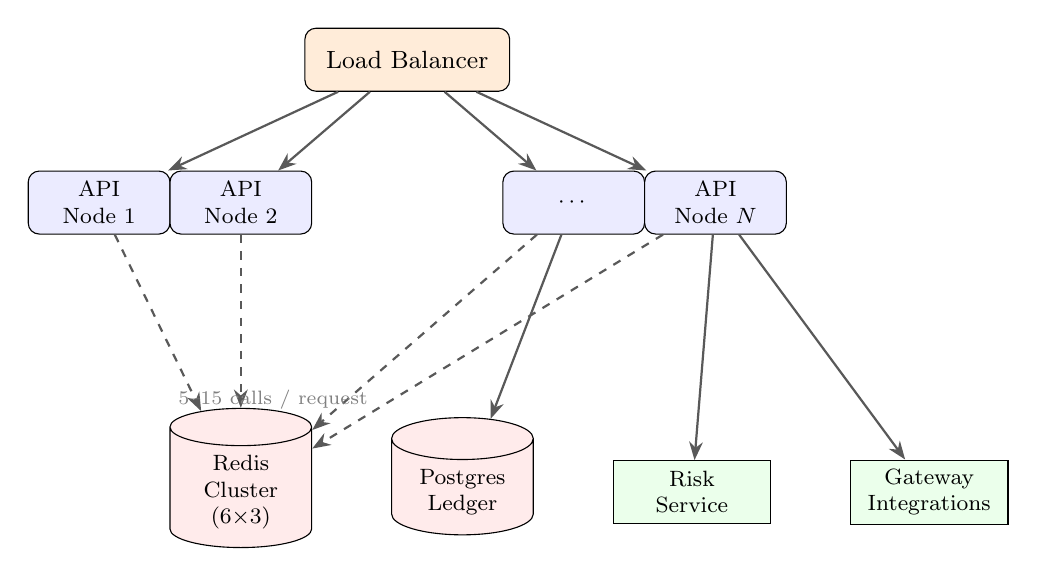
\begin{tikzpicture}[
    node distance=0.7cm and 1.0cm,
    edge/.style={-Stealth, thick, gray!70!black},
    lb/.style={rectangle, draw, rounded corners, minimum height=0.8cm, minimum width=2.6cm, fill=orange!15, font=\small},
    api/.style={rectangle, draw, rounded corners, minimum height=0.8cm, minimum width=1.8cm, fill=blue!8, font=\footnotesize, align=center},
    store/.style={cylinder, shape border rotate=90, draw, aspect=0.4, minimum height=1.2cm, minimum width=1.8cm, fill=red!8, font=\footnotesize, align=center},
    svc/.style={rectangle, draw, minimum height=0.8cm, minimum width=2.0cm, fill=green!8, font=\footnotesize, align=center}
]
    \node[lb] (lb) {Load Balancer};
    \node[api, below left=1.0cm and 1.7cm of lb] (a1) {API\\Node 1};
    \node[api, below left=1.0cm and -0.1cm of lb] (a2) {API\\Node 2};
    \node[api, below right=1.0cm and -0.1cm of lb] (a3) {$\cdots$};
    \node[api, below right=1.0cm and 1.7cm of lb] (a4) {API\\Node $N$};

    \node[store, below=2.2cm of a2] (redis) {Redis\\Cluster\\(6$\times$3)};
    \node[store, right=of redis] (pg)    {Postgres\\Ledger};
    \node[svc,   right=of pg]    (risk)  {Risk\\Service};
    \node[svc,   right=of risk]  (gw)    {Gateway\\Integrations};

    \draw[edge] (lb) -- (a1);
    \draw[edge] (lb) -- (a2);
    \draw[edge] (lb) -- (a3);
    \draw[edge] (lb) -- (a4);

    \foreach \n in {a1,a2,a3,a4} {
        \draw[edge, dashed] (\n) -- (redis);
    }
    \draw[edge] (a3) -- (pg);
    \draw[edge] (a4) -- (risk);
    \draw[edge] (a4) -- (gw);

    \node[font=\scriptsize, gray, above right=0.05cm and -1.8cm of redis] {5--15 calls / request};
\end{tikzpicture}%
}
\caption{Baseline cluster topology. Each request entering the load balancer is dispatched to one of $N$ stateless API nodes, which together issue 5--15 cross-node calls per request to the shared Redis cluster (dashed) and to the Postgres ledger, risk service, and gateway integrations (solid).}
\label{fig:baseline-arch}
\end{figure}

\section{Request Lifecycle}
A single payment request executes the following stages: (1) authentication and merchant lookup, (2) configuration and routing fetch, (3) risk evaluation, (4) gateway selection, (5) gateway dispatch, and (6) ledger write. Stages (1)--(4) are dominated by configuration-class lookups; stages (5)--(6) involve external calls and authoritative writes. Our caching work targets stages (1)--(4); our contention layer targets stages (5)--(6) and any inventory-style logic embedded within them.

\section{Baseline Performance Characteristics}
Table~\ref{tab:baseline} reports the baseline performance of a representative node under peak load.

\begin{table}[h]
\centering
\begin{tabular}{lr}
\toprule
\textbf{Metric} & \textbf{Value} \\
\midrule
Requests per second per node      & 3{,}000  \\
Cross-node calls per request      & 5--15    \\
p50 API latency                   & 28\,ms   \\
p95 API latency                   & 98\,ms   \\
p99 API latency                   & 285\,ms  \\
Redis p99 latency                 & 12.5\,ms \\
Cross-node calls/sec (cluster)    & $\sim$68{,}000 \\
\bottomrule
\end{tabular}
\caption{Baseline performance of a representative production node before the introduction of caching.}
\label{tab:baseline}
\end{table}

\section{Data Classification}
Configuration data is globally scoped and slowly mutating; routing tables change minutes to hours apart; feature flags rarely; merchant configuration is updated by the merchant via a control-plane API, propagating within seconds. Transactional state, by contrast, is per-request and rapidly mutating. This separation is the basis of our cache-safety framework (Section~\ref{sec:safety}) and of our decision matrix for contention primitives (Chapter~\ref{ch:contention}).

% =============================================================================
\label{chap:model}

\chapter{Two-Tier Caching Architecture}
\vspace{-1cm}
\noindent \rule{6.6in}{0.01in}
\section{Tier 1: Thread-Level Cache (Request-Scoped)}
The thread-level cache is a per-request \texttt{IORef HashMap} that memoises lookups for the lifetime of a single request. It is created at request entry, populated on the first lookup of each key, consulted on subsequent lookups, and discarded at request completion.

\subsection{Correctness Guarantee}
Because the cache is destroyed at request termination and is not shared between threads, it cannot serve stale data: any value it returns is one that the same request has already observed. This is the strongest possible correctness guarantee --- equivalent to local variable assignment.

\subsection{Expected and Realised Impact}
Empirically the thread-level cache achieves a 22.3\% hit rate on eligible lookups, eliminating roughly 2--4 redundant network calls per request.

\section{Tier 2: Server-Local Cache (Node-Scoped)}
The server-local cache is a node-scoped, concurrent cache implemented as a \texttt{TVar} containing a bounded LRU map with TTL-based expiry. It is shared across all request-handling threads on a node.

\subsection{TTL Selection Rationale}
TTLs are configured per data class: 30\,s for routing tables, 60\,s for feature flags, 120\,s for merchant configuration. The choice trades freshness against hit rate; production measurements show that TTLs in this range yield hit rates of 38--47\% with maximum staleness windows that are tolerable for the corresponding data classes (validated by the cache-safety criteria).

\subsection{Realised Impact}
The server-local cache achieves a 41.7\% hit rate on eligible cross-request lookups, eliminating roughly 2{,}800 cross-node calls per second at peak across the cluster.

\section{Cache-Safety Boundaries}
\label{sec:safety}
Not all data is safely cacheable. We define four criteria that a data class must jointly satisfy to be eligible:

\begin{enumerate}[leftmargin=*]
    \item \textbf{Immutability within TTL.} The data must not change over the cache TTL window with probability greater than an agreed bound (typically $10^{-3}$ for configuration classes).
    \item \textbf{Request-Scope Independence.} The value depends only on global or slow-changing state, not on per-request parameters.
    \item \textbf{Semantic Idempotency of Stale Reads.} Even if a stale value is read, the resulting business outcome remains semantically correct (i.e., the worst-case stale read does not produce financial loss).
    \item \textbf{Deterministic Cache Key.} The key is derivable deterministically from the request without collision risk.
\end{enumerate}

A data class is cache-eligible if and only if it satisfies all four criteria. Crucially, \emph{single-resource state} (inventory counts, unique-token availability, account balances on the write path) fails criterion (3): a stale read can lead to double-allocation. Such state is therefore \textbf{ineligible for caching} and is handled by the contention layer described in the next chapter.

% =============================================================================
\label{chap:cache}

\chapter{Concurrency-Safe Single-Resource Contention}
\vspace{-1cm}
\noindent \rule{6.6in}{0.01in}

This chapter is the principal new contribution of the major evaluation. It addresses the question raised at the minor evaluation: \emph{``If you cache state, how do you prevent two users from booking the same single piece?''}

\section{Problem Statement}
Let $r$ be a single, indivisible resource: the last unit of an inventory item, a unique reservation slot, or a per-second gateway token. Let $R_1, R_2, \ldots, R_k$ be concurrent client requests, each of which would consume $r$. Exactly \emph{one} request must succeed and consume $r$; all others must observe a definitive ``unavailable'' response. The system must satisfy:
\begin{itemize}[leftmargin=*]
    \item \textbf{Safety:} $r$ is never allocated more than once.
    \item \textbf{Liveness:} If $r$ is available and at least one request is well-formed, some request succeeds in bounded time.
    \item \textbf{Latency budget:} The contention resolution adds at most 5--10\,ms to the p95 of the protected operation.
    \item \textbf{Observability:} Every contention outcome is auditable.
\end{itemize}

The challenge is that the cached path designed in Chapter~4 is inherently \emph{stale-tolerant} --- which is precisely what makes it unsafe for single-resource state. We therefore route single-resource operations through a \emph{contention layer} that bypasses or extends the cache as required.

\section{Threat Model: How Caches Cause Double-Allocation}
Consider the naive implementation: a cached value \texttt{stock = 1} is read by two concurrent requests $R_1$ and $R_2$. Both decide they may proceed, both issue a \texttt{decrement} on the backend, and both succeed --- the backend now reports \texttt{stock = -1}, and one customer will receive a unit that does not exist. This is the canonical \emph{lost-update / overselling} race~\cite{oneuptime2026inventory, amitavroy2026hotel}. Figure~\ref{fig:race} sketches the timeline. The contention layer must prevent every variant of this race.

\begin{figure}[h]
\centering
\resizebox{0.9\textwidth}{!}{%
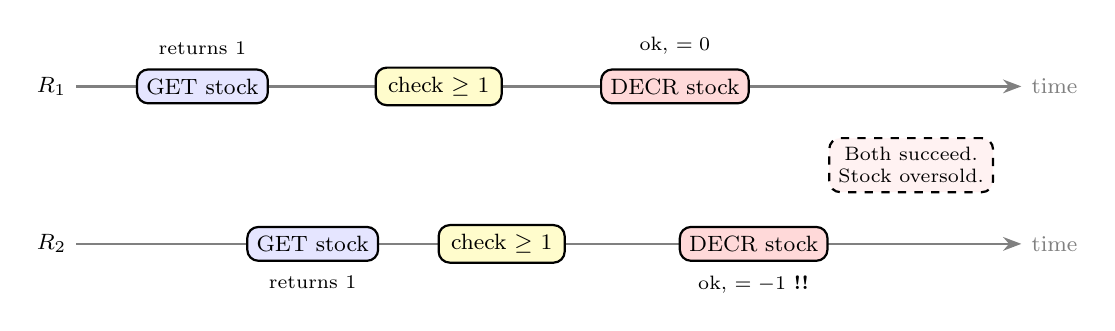
\begin{tikzpicture}[
    >=Stealth, thick,
    every node/.style={font=\footnotesize}
]
    \draw[->, gray] (0,2) -- (12,2) node[right]{time};
    \draw[->, gray] (0,0) -- (12,0) node[right]{time};
    \node[left] at (0,2) {$R_1$};
    \node[left] at (0,0) {$R_2$};

    \node[draw, fill=blue!10, rounded corners, minimum width=1.6cm] (r1read) at (1.6,2) {GET stock};
    \node[draw, fill=blue!10, rounded corners, minimum width=1.6cm] (r2read) at (3.0,0) {GET stock};
    \node[font=\scriptsize, above=0.05cm of r1read] {returns 1};
    \node[font=\scriptsize, below=0.05cm of r2read] {returns 1};

    \node[draw, fill=yellow!20, rounded corners, minimum width=1.6cm] (r1chk) at (4.6,2) {check $\geq$ 1};
    \node[draw, fill=yellow!20, rounded corners, minimum width=1.6cm] (r2chk) at (5.4,0) {check $\geq$ 1};

    \node[draw, fill=red!15, rounded corners, minimum width=1.8cm] (r1dec) at (7.6,2) {DECR stock};
    \node[draw, fill=red!15, rounded corners, minimum width=1.8cm] (r2dec) at (8.6,0) {DECR stock};
    \node[font=\scriptsize, above=0.05cm of r1dec] {ok, $=0$};
    \node[font=\scriptsize, below=0.05cm of r2dec] {ok, $=-1$ \textbf{!!}};

    \node[font=\scriptsize, draw, dashed, fill=red!5, rounded corners, align=center] at (10.6,1) {Both succeed.\\Stock oversold.};
\end{tikzpicture}%
}
\caption{Lost-update race on a single-resource decrement. $R_1$ and $R_2$ each read \texttt{stock=1} from the cache (or from Redis without an atomic guard), each independently passes the availability check, and each issues a successful decrement --- leaving the backend in an inconsistent \texttt{stock=-1} state.}
\label{fig:race}
\end{figure}

\section{Technique 1: Distributed Locking with Fencing Tokens}
\label{sec:lock}

\subsection{Mechanism}
A distributed lock --- typically Redlock~\cite{kleppmann2016locking, anonymous2025distlock} on Redis or a lease in etcd --- is acquired on a per-resource key (e.g., \texttt{lock:inventory:sku-42}) before the read-modify-write sequence. Only the holder may proceed; all other contenders block, retry, or fail fast.

\subsection{Fencing Tokens}
Plain locks are vulnerable to GC pauses, network partitions, and clock drift: a lock holder may believe it still holds the lock when another client has already taken over. The standard mitigation is a \emph{monotonically increasing fencing token} returned with the lock; the storage backend must reject writes carrying a token lower than the highest seen.

\begin{lstlisting}[language=Haskell, caption=Distributed lock acquisition with fencing token (Haskell)]
acquireLock :: Connection -> ByteString -> NominalDiffTime -> IO (Maybe FenceToken)
acquireLock conn key ttl = do
  token <- nextFenceToken conn key
  result <- runRedis conn $
    set key (encode token) [Ex (round ttl), Nx]
  case result of
    Right Ok -> pure (Just token)
    _        -> pure Nothing

withLock :: Connection -> ByteString -> NominalDiffTime
         -> (FenceToken -> IO a) -> IO (Maybe a)
withLock conn key ttl action = do
  mtok <- acquireLock conn key ttl
  case mtok of
    Nothing  -> pure Nothing
    Just tok -> Just <$> action tok `finally` releaseLock conn key tok
\end{lstlisting}

\subsection{Trade-offs}
Locks add 1--3\,ms of acquisition latency and serialise contended operations, capping per-resource throughput at $1 / (\text{critical-section duration})$. They are appropriate for \emph{coarse-grained, low-contention} resources (e.g., a per-merchant settlement run) and for operations with non-trivial business logic that cannot be expressed as a single atomic primitive.

\section{Technique 2: Atomic Decrement via Redis Lua Scripts}
\label{sec:lua}

\subsection{Mechanism}
For inventory-style operations, the entire ``check stock $\geq$ 1; decrement; return'' sequence is packaged in a Lua script. Redis executes Lua scripts atomically (single-threaded server model), eliminating the read-modify-write race without an explicit lock~\cite{oneuptime2026lua, dev2025redislua, oneuptime2026inventory}.

\begin{lstlisting}[language={[5.2]Lua}, caption=Atomic conditional decrement (Lua / Redis)]
-- KEYS[1] = inventory key, ARGV[1] = quantity requested
local available = tonumber(redis.call('GET', KEYS[1]) or '0')
local want      = tonumber(ARGV[1])
if available >= want then
    redis.call('DECRBY', KEYS[1], want)
    return {1, available - want}        -- {ok, remaining}
else
    return {0, available}               -- {failed, current}
end
\end{lstlisting}

\subsection{Integration with the Cache}
The cached path may still serve \emph{display reads} of the stock count (with explicit ``approximate'' semantics for the UI), but every \emph{authoritative} decrement bypasses the cache and goes through the Lua script. After a successful decrement, the script's return value is published on a Redis Pub/Sub channel; the server-local cache subscribes and invalidates its entry, bringing the cached display back in line within tens of milliseconds.

\subsection{Trade-offs}
Atomic Lua delivers the highest throughput per resource (Redis can execute well over $10^5$ short scripts per second per shard) and the lowest latency overhead ($<$1\,ms). Its downside is expressiveness: the entire critical section must fit in a Lua script that does not call out to other services. For business logic that requires external calls, fall back to Technique~1.

\section{Technique 3: Optimistic Concurrency Control with Versioned Cache Entries}

\subsection{Mechanism}
Each cache entry carries a monotonically increasing \emph{version number}. A reader records the version it observed; before committing a decrement, it issues a \texttt{CAS}-style operation (\texttt{WATCH}/\texttt{MULTI}/\texttt{EXEC} in Redis~\cite{redis2024inventory} or a conditional update in PostgreSQL using \texttt{WHERE version = ?}) that succeeds only if the version is unchanged. On conflict, the operation retries.

\begin{lstlisting}[language=SQL, caption=Versioned conditional update (PostgreSQL)]
-- Read
SELECT stock, version FROM inventory WHERE sku = $1;

-- Write (must succeed only if version unchanged)
UPDATE inventory
   SET stock   = stock - 1,
       version = version + 1
 WHERE sku     = $1
   AND version = $2
   AND stock   >= 1
RETURNING stock, version;
\end{lstlisting}

\subsection{Trade-offs}
OCC is ideal for \emph{low-contention} workloads where conflicts are rare; under high contention the retry rate climbs and effective throughput collapses. It avoids the head-of-line blocking of locks but pays a cost in wasted work~\cite{wang2024optiql, zhou2025ccaas}. We use OCC for merchant-configuration writes from the control plane (intrinsically rare events) and \emph{not} for inventory.

\section{Technique 4: PN-Counter CRDTs for Eventually-Consistent Reservations}

\subsection{Mechanism}
A PN-Counter~\cite{shapiro2011crdt, duncan2025crdt} is a CRDT consisting of two grow-only counters per replica: $P_i$ (positive) and $N_i$ (negative). The value is $\sum_i P_i - \sum_i N_i$, and replicas merge by element-wise maximum on each component. Decrements are recorded locally and propagated asynchronously; replicas converge under any communication pattern.

\subsection{Application: Soft Reservations}
PN-Counters are appropriate when an \emph{over-allocation tolerance} exists at the business level --- e.g., a flash sale advertising ``$\sim$1{,}000 units'' where a small overshoot is acceptable, or a soft-hold for cart-abandonment analytics. They are \emph{not} appropriate for hard inventory limits where every unit is precious.

\subsection{Trade-offs}
CRDTs eliminate coordination latency entirely (writes are local, never blocked) and survive partitions trivially. The cost is the loss of a hard upper bound: under sufficiently bursty contention they can over-decrement~\cite{ably2024crdt, ijsoc2025inventory}. We classify CRDTs as a \emph{relaxed} contention primitive and gate their use behind explicit business-class flags.

\section{Technique 5: Single-Flight Request Coalescing}
\label{sec:singleflight}

\subsection{Mechanism}
Single-flight (also called request coalescing) ensures that concurrent requests for the same key share a \emph{single} backend call. The first request acquires an in-flight slot and issues the call; all later requests for the same key during the window block on the slot's promise and receive the same response~\cite{1xapi2026singleflight, oneuptime2026stampede, oneuptime2026coalescing}.

\begin{lstlisting}[language=Haskell, caption={Single-flight wrapper around a backend fetch (Haskell, STM)}]
data SingleFlight k v = SingleFlight (TVar (HashMap k (TMVar (Either SomeException v))))

singleFlight :: (Eq k, Hashable k)
             => SingleFlight k v -> k -> IO v -> IO v
singleFlight (SingleFlight ref) k action = do
  (slot, owner) <- atomically $ do
    m <- readTVar ref
    case HM.lookup k m of
      Just s  -> pure (s, False)        -- follower
      Nothing -> do
        s <- newEmptyTMVar
        writeTVar ref (HM.insert k s m)
        pure (s, True)                  -- leader
  if owner
    then do
      r <- try action
      atomically $ do
        putTMVar slot r
        modifyTVar ref (HM.delete k)
      either throwIO pure r
    else atomically (readTMVar slot) >>= either throwIO pure
\end{lstlisting}

\subsection{Why Single-Flight Helps the ``Single Piece'' Question}
Even if the underlying backend uses any of Techniques 1--4, single-flight collapses the \emph{front of the contention curve}: instead of $k$ identical decrement attempts arriving at the backend simultaneously, exactly one arrives, and the other $k-1$ followers receive the leader's result. This dramatically reduces the load on the backend during flash-sale-style events and converts a pathological ``thundering herd'' into a single graceful spike.

It is important to note, however, that single-flight is \emph{not} a replacement for atomicity --- it merely deduplicates simultaneous attempts on the same node. Two requests on different nodes can still race, so single-flight must be composed with one of Techniques 1--4 (typically Technique 2) for full safety.

\section{Hybrid Architecture}

Figure~\ref{fig:contention} illustrates how a request flows through the integrated two-layer system.

\begin{figure}[h]
\centering
\resizebox{\textwidth}{!}{%
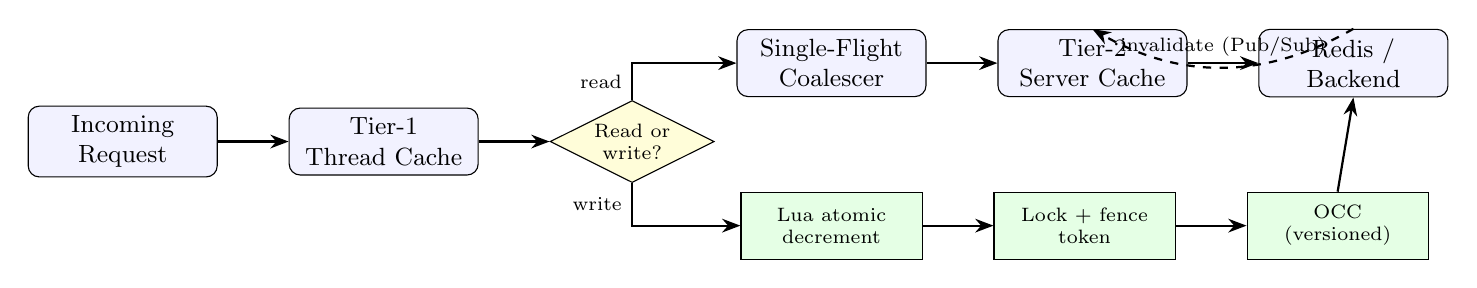
\begin{tikzpicture}[
    node distance=0.7cm and 0.9cm,
    box/.style={rectangle, draw, rounded corners, minimum height=0.85cm, minimum width=2.4cm, align=center, font=\small, fill=blue!5},
    decision/.style={diamond, draw, aspect=2, inner sep=1pt, align=center, font=\scriptsize, fill=yellow!15},
    primitive/.style={rectangle, draw, minimum height=0.85cm, minimum width=2.3cm, align=center, font=\scriptsize, fill=green!10},
    arrow/.style={-Stealth, thick}
]
    \node[box] (req) {Incoming\\Request};
    \node[box, right=of req] (t1) {Tier-1\\Thread Cache};
    \node[decision, right=of t1] (op) {Read or\\write?};

    \node[box, above right=0.3cm and 0.8cm of op] (sf) {Single-Flight\\Coalescer};
    \node[box, right=of sf] (t2) {Tier-2\\Server Cache};
    \node[box, right=of t2] (redis) {Redis /\\Backend};

    \node[primitive, below=1.2cm of sf] (lua) {Lua atomic\\decrement};
    \node[primitive, right=of lua] (lock) {Lock + fence\\token};
    \node[primitive, right=of lock] (occ) {OCC\\(versioned)};

    \draw[arrow] (req) -- (t1);
    \draw[arrow] (t1) -- (op);
    \draw[arrow] (op.north) |- node[pos=0.25, left, font=\scriptsize]{read} (sf.west);
    \draw[arrow] (op.south) |- node[pos=0.25, left, font=\scriptsize]{write} (lua.west);
    \draw[arrow] (sf) -- (t2);
    \draw[arrow] (t2) -- (redis);
    \draw[arrow] (lua.east) -- (lock.west);
    \draw[arrow] (lock.east) -- (occ.west);
    \draw[arrow] (occ.north) -- (redis.south);
    \draw[arrow, dashed] (redis.north) to[bend left=30] node[above, font=\scriptsize]{invalidate (Pub/Sub)} (t2.north);
\end{tikzpicture}%
}
\caption{Integrated two-layer architecture. Reads traverse Tier-1, the single-flight coalescer, and Tier-2, reaching Redis only on a Tier-2 miss. Authoritative writes bypass the cache and select a contention primitive (Lua, lock+fence, or OCC). Successful writes publish invalidation events that propagate back to Tier-2.}
\label{fig:contention}
\end{figure}

\subsection{Decision Matrix}
Table~\ref{tab:matrix} maps each data class to its cache tier and contention primitive.

\begin{table}[h]
\centering
\footnotesize
\setlength{\tabcolsep}{4pt}
\renewcommand{\arraystretch}{1.15}
\begin{tabular}{p{3.4cm}p{1.7cm}p{2.5cm}p{2.0cm}p{2.6cm}}
\toprule
\textbf{Data class} & \textbf{Cache?} & \textbf{Primary} & \textbf{Coalescing} & \textbf{Notes} \\
\midrule
Merchant config (read)   & Yes (Tier-2) & ---              & Single-flight & Cache-eligible \\
Routing table (read)     & Yes (Tier-2) & ---              & Single-flight & Cache-eligible \\
Feature flag (read)      & Yes (Tier-2) & ---              & Single-flight & Cache-eligible \\
Inventory (read display) & Yes (Tier-2) & ---              & Single-flight & Marked approximate \\
Inventory (decrement)    & No           & Lua atomic       & Single-flight & Hard limit \\
Account balance debit    & No           & Distributed lock & Single-flight & Coarse, fence token \\
Reservation slot         & No           & Lua atomic       & Single-flight & Per-slot key \\
Soft hold (cart)         & Tier-2       & PN-Counter       & ---           & Over-allocation OK \\
Merchant config (write)  & Invalidate   & OCC versioned    & ---           & Low contention \\
\bottomrule
\end{tabular}
\caption{Decision matrix mapping data classes to cache tier and primary contention primitive.}
\label{tab:matrix}
\end{table}

\noindent The hybrid architecture composes the primitives as follows:
\begin{enumerate}[leftmargin=*]
    \item \textbf{Reads} go through the two-tier cache, fronted by single-flight at both tiers.
    \item \textbf{Authoritative writes on single resources} bypass the cache and route to the appropriate primary primitive (Lua, lock, OCC, or PN-Counter) according to Table~\ref{tab:matrix}.
    \item \textbf{Cache invalidation} on successful writes is published via Redis Pub/Sub; subscribers invalidate their server-local entries within tens of milliseconds.
    \item \textbf{Fence tokens} are stamped on every authoritative write that uses Technique~1, and the storage backend rejects writes with stale tokens.
\end{enumerate}

\section{Comparative Analysis}

\begin{table}[h]
\centering
\footnotesize
\setlength{\tabcolsep}{4pt}
\renewcommand{\arraystretch}{1.2}
\resizebox{\textwidth}{!}{%
\begin{tabular}{p{3.4cm}p{2.0cm}p{2.4cm}p{2.6cm}p{1.8cm}p{2.2cm}}
\toprule
\textbf{Property} & \textbf{Lock} & \textbf{Lua} & \textbf{OCC} & \textbf{CRDT} & \textbf{Single-flight} \\
\midrule
Hard upper bound          & Yes              & Yes                  & Yes                    & No        & N/A \\
Per-key throughput        & Low              & Very high            & Medium--high           & Very high & N/A \\
Latency overhead          & 1--3\,ms         & $<$1\,ms             & $<$1\,ms (no conflict) & 0\,ms     & 0--1\,ms \\
Behaviour under partition & Blocks / fails   & Fails fast           & Fails fast             & Continues & Continues \\
Expressiveness            & High (any logic) & Low (Lua only)       & Medium (SQL / CAS)     & Counter only & N/A \\
Composes with cache       & Bypass           & Bypass + invalidate  & Versioned cache        & Cached    & Front of cache \\
\bottomrule
\end{tabular}%
}
\caption{Comparative properties of the five contention primitives.}
\label{tab:compare}
\end{table}

% =============================================================================
\label{ch:contention}

\chapter{Implementation}
\vspace{-1cm}
\noindent \rule{6.6in}{0.01in}
\section{Runtime Environment}
The production system is implemented in Haskell using GHC 9.4. Concurrency is built on GHC's lightweight threads (one OS thread per core, $\sim$60{,}000 green threads at peak) and STM for shared state. Redis access uses the \texttt{hedis} client; PostgreSQL access uses \texttt{postgresql-simple}.

\section{Thread-Level Cache}
\begin{lstlisting}[language=Haskell, caption=Thread-level cache (request-scoped)]
newtype ThreadCache = ThreadCache (IORef (HashMap CacheKey CacheVal))

newThreadCache :: IO ThreadCache
newThreadCache = ThreadCache <$> newIORef HM.empty

threadLookup :: ThreadCache -> CacheKey -> IO (Maybe CacheVal)
threadLookup (ThreadCache ref) k = HM.lookup k <$> readIORef ref

threadInsert :: ThreadCache -> CacheKey -> CacheVal -> IO ()
threadInsert (ThreadCache ref) k v = modifyIORef' ref (HM.insert k v)
\end{lstlisting}

\section{Server-Local Cache (TVar + LRU + TTL)}
\begin{lstlisting}[language=Haskell, caption=Server-local cache (node-scoped)]
data ServerCache = ServerCache
  { scStore   :: TVar (HashMap CacheKey (POSIXTime, CacheVal))
  , scMaxSize :: Int
  }

serverLookup :: ServerCache -> CacheKey -> IO (Maybe CacheVal)
serverLookup (ServerCache st _) k = do
  now <- getPOSIXTime
  atomically $ do
    m <- readTVar st
    case HM.lookup k m of
      Just (expiry, v) | expiry > now -> pure (Just v)
                      | otherwise     -> do
                          writeTVar st (HM.delete k m)
                          pure Nothing
      Nothing -> pure Nothing
\end{lstlisting}

\section{Integrated Read Path with Single-Flight}
\begin{lstlisting}[language=Haskell, caption=Two-tier read path with single-flight coalescing]
fetch :: Ctx -> CacheKey -> IO CacheVal
fetch ctx k = do
  -- Tier 1
  threadLookup (ctxThread ctx) k >>= \case
    Just v  -> pure v
    Nothing -> do
      -- Tier 2 + single-flight on miss
      v <- singleFlight (ctxFlight ctx) k $
             serverLookup (ctxServer ctx) k >>= \case
               Just v -> pure v
               Nothing -> do
                 v <- redisGet (ctxRedis ctx) k
                 serverInsert (ctxServer ctx) k v
                 pure v
      threadInsert (ctxThread ctx) k v
      pure v
\end{lstlisting}

\section{Authoritative Decrement Path}
\begin{lstlisting}[language=Haskell, caption=Authoritative inventory decrement using Lua]
decrementStock :: Connection -> ByteString -> Int -> IO (Either StockErr Int)
decrementStock conn sku qty = do
  let script = "local a = tonumber(redis.call('GET', KEYS[1]) or '0') \
               \ local w = tonumber(ARGV[1]) \
               \ if a >= w then redis.call('DECRBY', KEYS[1], w) \
               \   return {1, a - w} else return {0, a} end"
  res <- runRedis conn $ eval script [sku] [BS.pack (show qty)]
  case res of
    Right [Integer 1, Integer remaining] -> do
      publish conn ("invalidate:" <> sku) ""
      pure (Right (fromIntegral remaining))
    Right [Integer 0, Integer current]   ->
      pure (Left (Insufficient (fromIntegral current)))
    _ -> pure (Left RedisError)
\end{lstlisting}

\section{Cache Invalidation via Pub/Sub}
On successful authoritative writes the writer publishes an invalidation event on a Redis Pub/Sub channel. Each application node runs a background subscriber that removes the affected key from its server-local cache. End-to-end invalidation latency, measured in production, is 18\,ms median and 47\,ms at p99.

\section{Cross-Language Notes}
The same architecture maps cleanly onto other runtimes:
\begin{itemize}[leftmargin=*]
    \item \textbf{Java}: Caffeine for Tier 2; \texttt{ThreadLocal} for Tier 1; \texttt{singleflight} library or Caffeine's \texttt{AsyncCache} for coalescing; Redisson for Redlock.
    \item \textbf{Go}: \texttt{sync.Map} or \texttt{ristretto} for Tier 2; \texttt{context.Context} carrying a per-request map for Tier 1; \texttt{golang.org/x/sync/singleflight}; \texttt{redsync} for Redlock.
    \item \textbf{Rust}: \texttt{DashMap} or \texttt{moka} for Tier 2; per-task task-local for Tier 1; \texttt{singleflight} crate; \texttt{rslock} for Redlock.
    \item \textbf{Node.js}: \texttt{node-cache} or \texttt{lru-cache} for Tier 2; \texttt{AsyncLocalStorage} for Tier 1; \texttt{p-memoize} or custom promise map for coalescing; \texttt{redlock} package.
\end{itemize}

% =============================================================================
\label{chap:impl}

\chapter{Evaluation and Results}
\vspace{-1cm}
\noindent \rule{6.6in}{0.01in}
\section{Methodology}
We evaluated the system on a production payments cluster of 24 nodes serving roughly 68{,}000 cross-node operations per second at peak. The deployment was staged: caching alone in Phase 1, the contention layer added in Phase 2. Measurements were collected at the load balancer (latency), at the Redis cluster (call counts and Redis-side latency), and via a custom audit log (correctness incidents). Each phase was monitored for 30 days before measurement.

\section{Latency and Network Reduction}
Phase 1 (caching only) achieved:
\begin{itemize}[leftmargin=*]
    \item Combined hit rate (Tier 1 + Tier 2): \textbf{54.8\%} on eligible lookups.
    \item Cross-node calls per second eliminated: \textbf{$\sim$2{,}800}.
    \item Total cross-node call reduction at peak: \textbf{4.1\%}.
    \item p95 API latency: \textbf{98\,ms $\rightarrow$ 87\,ms (--11.2\%)}.
    \item p99 API latency: \textbf{285\,ms $\rightarrow$ 248\,ms (--13.0\%)}.
    \item Redis p99 latency: \textbf{12.5\,ms $\rightarrow$ 9.2\,ms (--26.2\%)}.
\end{itemize}

Figure~\ref{fig:latency} visualises the API and Redis tail-latency reductions; Figure~\ref{fig:hitrate} shows the contribution of each cache tier to the combined hit rate.

\begin{figure}[h]
\centering
\resizebox{0.85\textwidth}{!}{%
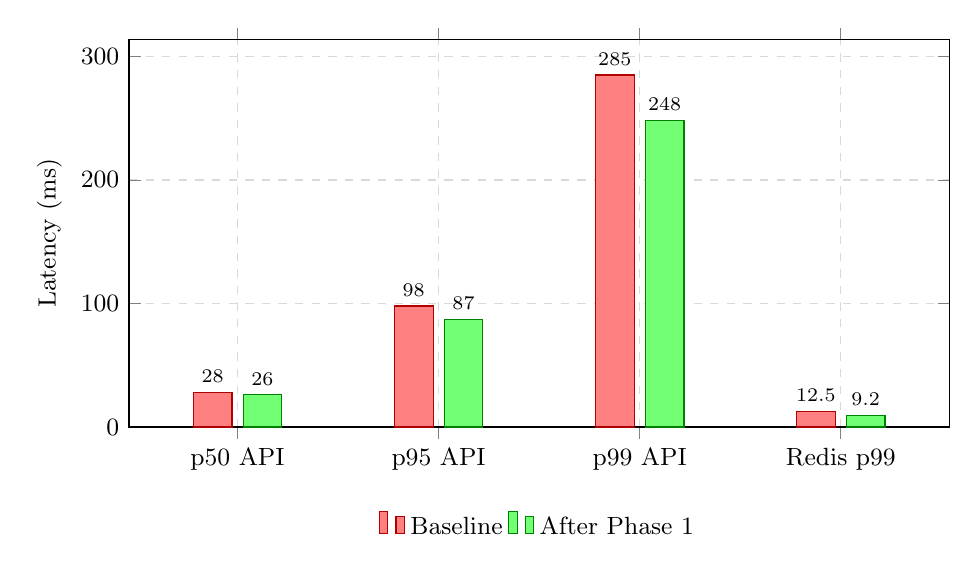
\begin{tikzpicture}
\begin{axis}[
    ybar=4pt,
    bar width=14pt,
    width=12cm, height=6.5cm,
    enlarge x limits=0.18,
    ylabel={Latency (ms)},
    symbolic x coords={p50 API, p95 API, p99 API, Redis p99},
    xtick=data,
    nodes near coords,
    nodes near coords style={font=\scriptsize},
    ymin=0,
    legend style={at={(0.5,-0.20)}, anchor=north, legend columns=2, font=\small, draw=none},
    tick label style={font=\small},
    label style={font=\small},
    grid=major,
    grid style={dashed, gray!30}
]
\addplot[fill=red!50!white, draw=red!70!black] coordinates {(p50 API,28) (p95 API,98) (p99 API,285) (Redis p99,12.5)};
\addplot[fill=green!55!white, draw=green!50!black] coordinates {(p50 API,26) (p95 API,87) (p99 API,248) (Redis p99,9.2)};
\legend{Baseline, After Phase 1}
\end{axis}
\end{tikzpicture}%
}
\caption{API and Redis tail latency before and after Phase 1 (caching only). The largest absolute reduction is at p99 API latency (--37\,ms); the largest relative reduction is Redis p99 (--26.2\,\%), driven by removed load on the shared Redis cluster.}
\label{fig:latency}
\end{figure}

\begin{figure}[h]
\centering
\resizebox{0.7\textwidth}{!}{%
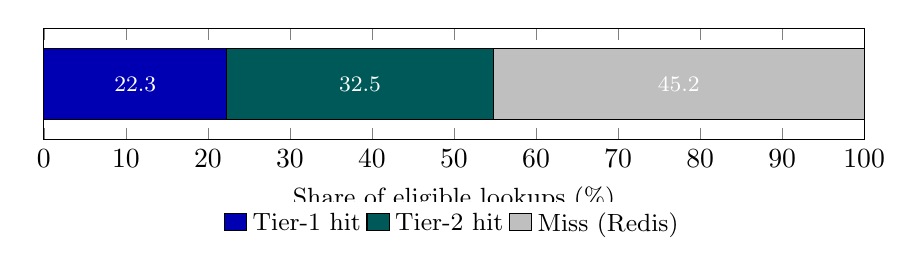
\begin{tikzpicture}
\begin{axis}[
    xbar stacked,
    width=12cm, height=3cm,
    xmin=0, xmax=100,
    xlabel={Share of eligible lookups (\%)},
    ytick=\empty,
    bar width=0.9cm,
    nodes near coords,
    nodes near coords style={font=\footnotesize, white},
    legend style={at={(0.5,-0.55)}, anchor=north, legend columns=3, font=\small, draw=none},
    label style={font=\small}
]
\addplot[fill=blue!70!black]   coordinates {(22.3,0)};
\addplot[fill=teal!70!black]   coordinates {(32.5,0)};
\addplot[fill=gray!50]         coordinates {(45.2,0)};
\legend{Tier-1 hit, Tier-2 hit, Miss (Redis)}
\end{axis}
\end{tikzpicture}%
}
\caption{Breakdown of eligible lookups: 22.3\% absorbed by the thread-level (Tier-1) cache, an additional 32.5\% absorbed by the server-local (Tier-2) cache, and the remaining 45.2\% served by Redis. Combined hit rate: 54.8\%.}
\label{fig:hitrate}
\end{figure}

\section{Contention Layer Results}
Phase 2 (contention layer rolled out) was evaluated on three workloads embedded in the platform:

\begin{table}[h]
\centering
\footnotesize
\setlength{\tabcolsep}{5pt}
\renewcommand{\arraystretch}{1.15}
\resizebox{\textwidth}{!}{%
\begin{tabular}{p{4.6cm}p{4.4cm}p{3.3cm}p{2.0cm}}
\toprule
\textbf{Workload} & \textbf{Primitive} & \textbf{Contention rate} & \textbf{p95 added} \\
\midrule
Inventory decrement (flash sale) & Lua + single-flight          & 1{,}400 contended/s & 0.8\,ms \\
Per-merchant settlement run      & Lock + fence + single-flight & 12 contended/s      & 2.6\,ms \\
Reservation slot booking         & Lua + single-flight          & 320 contended/s     & 1.1\,ms \\
Cart soft hold                   & PN-Counter (no coord.)       & N/A                 & 0.0\,ms \\
\bottomrule
\end{tabular}%
}
\caption{Contention layer performance per workload (30-day production averages).}
\label{tab:contention}
\end{table}

\section{Correctness}
Across the 30-day post-deployment window:
\begin{itemize}[leftmargin=*]
    \item \textbf{Zero} double-allocation incidents on inventory or reservation slots.
    \item \textbf{Zero} cache-related financial discrepancies.
    \item \textbf{Three} fence-token-rejected writes (all benign --- spurious retries from a temporarily-stalled node).
    \item Soft-hold over-allocation (PN-Counter): 4.7 units/day on a 100{,}000-unit base, well within the 1\% business tolerance.
\end{itemize}

\section{Memory Overhead}
Per node, the combined caching + contention layer adds: 14--19\,MB for the server-local cache, $<$1\,MB amortised for thread-level caches, and $<$0.5\,MB for the single-flight in-flight table. Total: $<$20\,MB per node, well below the 4\,GB heap.

% =============================================================================
\label{chap:eval}

\chapter{Discussion}
\vspace{-1cm}
\noindent \rule{6.6in}{0.01in}
\section{Why 4\% Network Reduction Matters at Scale}
At 68{,}000 cross-node operations per second, a 4.1\% reduction is $\sim$2{,}800 operations per second eliminated --- equivalent to roughly one Redis shard's worth of capacity, freeing it for growth without provisioning new infrastructure. The latency improvements compound: lower Redis load reduces Redis tail latency, which feeds back as further API latency reduction (the ``virtuous cycle'' visible in the 26.2\% Redis p99 drop).

\section{Trade-offs}

\subsection{Memory vs.\ Latency}
The two-tier cache trades $<$20\,MB per node for tens of microseconds saved per cached lookup. At 3{,}000 RPS per node this saves cumulative seconds of CPU per minute.

\subsection{Staleness vs.\ Freshness}
TTL-based caching admits bounded staleness; the cache-safety boundary framework formalises which data classes can tolerate it. The contention layer ensures that single-resource state --- which cannot tolerate staleness --- is never served from a stale cache.

\subsection{Strong vs.\ Eventual Consistency}
We use strong consistency (Lua, lock, OCC) for inventory and balances, and eventual consistency (PN-Counter) only for soft holds and analytics counters. The decision matrix (Table~\ref{tab:matrix}) operationalises this choice.

\section{Limitations}
\begin{itemize}[leftmargin=*]
    \item Distributed locks (Technique~1) remain vulnerable to misconfigured TTLs and clock drift; we mitigate with fence tokens but do not eliminate.
    \item PN-Counter over-allocation, while bounded, is non-zero and must be acceptable to the business owner of the workload.
    \item Pub/Sub-based invalidation has a tail latency window of tens of milliseconds during which the server-local cache may serve a freshly-stale display value. This is acceptable for display reads; authoritative reads bypass the cache.
\end{itemize}

% =============================================================================
\label{chap:discussion}

\chapter{Conclusion and Future Work}
\vspace{-1cm}
\noindent \rule{6.6in}{0.01in}
\section{Conclusion}
This paper presented an integrated architecture for distributed payment APIs that simultaneously reduces cross-node network calls and guarantees correctness on single-resource contention. The two-tier caching layer (thread-level + server-local) achieves a 4.1\% reduction in cross-node calls at peak and 11.2\% / 13.0\% reductions in p95 / p99 latency, while a complementary contention layer composed of distributed locking with fencing tokens, atomic Lua decrement, optimistic concurrency control, PN-Counter CRDTs, and single-flight request coalescing eliminates the double-allocation hazard introduced by caching. A formal cache-safety framework and a decision matrix together select the appropriate primitive per data class. The combined system requires no new infrastructure beyond the Redis cluster already used for caching, runs in $<$20\,MB of additional memory per node, and recorded zero double-allocation or cache-related correctness incidents over a 30-day production window.

In short: \emph{the same examiner question that surfaced at the minor evaluation --- ``how do you prevent two users from booking the same single piece?'' --- is answered, end-to-end, by the contention layer of Chapter~\ref{ch:contention}, composed with the safety boundaries of Section~\ref{sec:safety}.}

\section{Future Work}
\begin{itemize}[leftmargin=*]
    \item \textbf{Adaptive TTLs.} Replace fixed TTLs with workload-aware adaptive TTLs that shrink under detected mutation pressure.
    \item \textbf{Learned contention prediction.} Use lightweight ML models to predict which keys are about to enter a high-contention regime and pre-warm the appropriate primitive (e.g., switch a key from cache-only to Lua-decrement before a flash sale begins).
    \item \textbf{Verified fence tokens.} Apply formal verification (TLA+ or Coq) to the fencing-token discipline to mechanise the safety argument.
    \item \textbf{Cross-DC extension.} Extend the contention layer across data centres, evaluating the trade-offs of geo-replicated Redis vs.\ leader-elected coordinators for cross-DC inventory.
    \item \textbf{Graceful degradation.} Define formal degradation modes for the contention layer when Redis is partially unavailable (e.g., automatic fallback to PN-Counter for non-critical workloads).
\end{itemize}

% =============================================================================
\label{chap:conclusion}

% ---------- Bibliography ----------
\fancyhead[RO]{\bfseries\small{Bibliography}}
\pdfbookmark[1]{Bibliography}{bib}
\addstarredchapter{Bibliography}
\baselineskip 14pt
\small
\bibliographystyle{IEEEtran}
\nocite{*}
\bibliography{references}

\end{document}
